%% Pattern Recognition Letters version of ../paper/main.tex.
%% Template: Elsevier elsarticle.cls + prletters.sty (PRL style file), author-year references.
%% Build: latexmk -pdf main.tex   (or pdflatex, bibtex, pdflatex, pdflatex)
\documentclass[times,twocolumn,final,authoryear]{elsarticle}

\usepackage{prletters}
\usepackage[utf8]{inputenc}
\usepackage[T1]{fontenc}
\usepackage{amsmath,amssymb}
\usepackage{booktabs}
\usepackage{graphicx}
\usepackage{url}
\IfFileExists{letltxmacro.sty}{\usepackage[hidelinks]{hyperref}}{}

\setlength{\textfloatsep}{8pt plus 2pt minus 2pt}
\setlength{\floatsep}{6pt plus 2pt minus 2pt}
\setlength{\dbltextfloatsep}{8pt plus 2pt minus 2pt}

% Every number from a result is a macro from numbers.tex, a copy of ../paper/numbers.tex, which
% ../paper/make_tables.py writes from the CSVs in ../experiments/. The tables in tables/ are copies of
% ../paper/tables/; the figures are drawn by make_figures.py (this folder) from the same CSVs.
% Generated by make_tables.py from the CSVs in ../experiments/. Do not edit.
\newcommand{\gainInOrderAll}{\ensuremath{+0.100}}
\newcommand{\gainInOrderAllSE}{\ensuremath{0.006}}
\newcommand{\gainInOrderAllPM}{\ensuremath{+0.100 \pm 0.006}}
\newcommand{\gainShuffledAll}{\ensuremath{+0.062}}
\newcommand{\gainShuffledAllSE}{\ensuremath{0.003}}
\newcommand{\gainShuffledAllPM}{\ensuremath{+0.062 \pm 0.003}}
\newcommand{\localityAll}{\ensuremath{+0.038}}
\newcommand{\localityAllSE}{\ensuremath{0.004}}
\newcommand{\localityAllPM}{\ensuremath{+0.038 \pm 0.004}}
\newcommand{\gainUnigramAll}{\ensuremath{+0.018}}
\newcommand{\gainUnigramAllSE}{\ensuremath{0.004}}
\newcommand{\gainUnigramAllPM}{\ensuremath{+0.018 \pm 0.004}}
\newcommand{\inOrderMinusUnigramAll}{\ensuremath{+0.082}}
\newcommand{\inOrderMinusUnigramAllSE}{\ensuremath{0.004}}
\newcommand{\inOrderMinusUnigramAllPM}{\ensuremath{+0.082 \pm 0.004}}
\newcommand{\shuffledShareAll}{62\%}
\newcommand{\gainInOrderSameChunk}{\ensuremath{-0.111}}
\newcommand{\gainInOrderSameChunkSE}{\ensuremath{0.014}}
\newcommand{\gainInOrderSameChunkPM}{\ensuremath{-0.111 \pm 0.014}}
\newcommand{\gainShuffledSameChunk}{\ensuremath{-0.133}}
\newcommand{\gainShuffledSameChunkSE}{\ensuremath{0.010}}
\newcommand{\gainShuffledSameChunkPM}{\ensuremath{-0.133 \pm 0.010}}
\newcommand{\localitySameChunk}{\ensuremath{+0.022}}
\newcommand{\localitySameChunkSE}{\ensuremath{0.013}}
\newcommand{\localitySameChunkPM}{\ensuremath{+0.022 \pm 0.013^{\dagger}}}
\newcommand{\gainUnigramSameChunk}{\ensuremath{+0.096}}
\newcommand{\gainUnigramSameChunkSE}{\ensuremath{0.017}}
\newcommand{\gainUnigramSameChunkPM}{\ensuremath{+0.096 \pm 0.017}}
\newcommand{\inOrderMinusUnigramSameChunk}{\ensuremath{-0.206}}
\newcommand{\inOrderMinusUnigramSameChunkSE}{\ensuremath{0.022}}
\newcommand{\inOrderMinusUnigramSameChunkPM}{\ensuremath{-0.206 \pm 0.022}}
\newcommand{\gainInOrderOneK}{\ensuremath{+0.307}}
\newcommand{\gainInOrderOneKSE}{\ensuremath{0.011}}
\newcommand{\gainInOrderOneKPM}{\ensuremath{+0.307 \pm 0.011}}
\newcommand{\gainShuffledOneK}{\ensuremath{+0.062}}
\newcommand{\gainShuffledOneKSE}{\ensuremath{0.007}}
\newcommand{\gainShuffledOneKPM}{\ensuremath{+0.062 \pm 0.007}}
\newcommand{\localityOneK}{\ensuremath{+0.245}}
\newcommand{\localityOneKSE}{\ensuremath{0.009}}
\newcommand{\localityOneKPM}{\ensuremath{+0.245 \pm 0.009}}
\newcommand{\gainUnigramOneK}{\ensuremath{+0.461}}
\newcommand{\gainUnigramOneKSE}{\ensuremath{0.024}}
\newcommand{\gainUnigramOneKPM}{\ensuremath{+0.461 \pm 0.024}}
\newcommand{\inOrderMinusUnigramOneK}{\ensuremath{-0.154}}
\newcommand{\inOrderMinusUnigramOneKSE}{\ensuremath{0.026}}
\newcommand{\inOrderMinusUnigramOneKPM}{\ensuremath{-0.154 \pm 0.026}}
\newcommand{\shuffledShareOneK}{20\%}
\newcommand{\gainInOrderTenK}{\ensuremath{+0.144}}
\newcommand{\gainInOrderTenKSE}{\ensuremath{0.008}}
\newcommand{\gainInOrderTenKPM}{\ensuremath{+0.144 \pm 0.008}}
\newcommand{\gainShuffledTenK}{\ensuremath{+0.035}}
\newcommand{\gainShuffledTenKSE}{\ensuremath{0.005}}
\newcommand{\gainShuffledTenKPM}{\ensuremath{+0.035 \pm 0.005}}
\newcommand{\localityTenK}{\ensuremath{+0.109}}
\newcommand{\localityTenKSE}{\ensuremath{0.006}}
\newcommand{\localityTenKPM}{\ensuremath{+0.109 \pm 0.006}}
\newcommand{\gainUnigramTenK}{\ensuremath{+0.059}}
\newcommand{\gainUnigramTenKSE}{\ensuremath{0.007}}
\newcommand{\gainUnigramTenKPM}{\ensuremath{+0.059 \pm 0.007}}
\newcommand{\inOrderMinusUnigramTenK}{\ensuremath{+0.085}}
\newcommand{\inOrderMinusUnigramTenKSE}{\ensuremath{0.008}}
\newcommand{\inOrderMinusUnigramTenKPM}{\ensuremath{+0.085 \pm 0.008}}
\newcommand{\shuffledShareTenK}{24\%}
\newcommand{\gainInOrderHundredK}{\ensuremath{+0.009}}
\newcommand{\gainInOrderHundredKSE}{\ensuremath{0.006}}
\newcommand{\gainInOrderHundredKPM}{\ensuremath{+0.009 \pm 0.006^{\dagger}}}
\newcommand{\gainShuffledHundredK}{\ensuremath{+0.026}}
\newcommand{\gainShuffledHundredKSE}{\ensuremath{0.005}}
\newcommand{\gainShuffledHundredKPM}{\ensuremath{+0.026 \pm 0.005}}
\newcommand{\localityHundredK}{\ensuremath{-0.017}}
\newcommand{\localityHundredKSE}{\ensuremath{0.006}}
\newcommand{\localityHundredKPM}{\ensuremath{-0.017 \pm 0.006}}
\newcommand{\gainUnigramHundredK}{\ensuremath{-0.051}}
\newcommand{\gainUnigramHundredKSE}{\ensuremath{0.000}}
\newcommand{\gainUnigramHundredKPM}{\ensuremath{-0.051 \pm 0.000}}
\newcommand{\inOrderMinusUnigramHundredK}{\ensuremath{+0.060}}
\newcommand{\inOrderMinusUnigramHundredKSE}{\ensuremath{0.006}}
\newcommand{\inOrderMinusUnigramHundredKPM}{\ensuremath{+0.060 \pm 0.006}}
\newcommand{\gainInOrderFar}{\ensuremath{-0.039}}
\newcommand{\gainInOrderFarSE}{\ensuremath{0.009}}
\newcommand{\gainInOrderFarPM}{\ensuremath{-0.039 \pm 0.009}}
\newcommand{\gainShuffledFar}{\ensuremath{-0.017}}
\newcommand{\gainShuffledFarSE}{\ensuremath{0.008}}
\newcommand{\gainShuffledFarPM}{\ensuremath{-0.017 \pm 0.008}}
\newcommand{\localityFar}{\ensuremath{-0.023}}
\newcommand{\localityFarSE}{\ensuremath{0.008}}
\newcommand{\localityFarPM}{\ensuremath{-0.023 \pm 0.008}}
\newcommand{\gainUnigramFar}{\ensuremath{-0.051}}
\newcommand{\gainUnigramFarSE}{\ensuremath{0.000}}
\newcommand{\gainUnigramFarPM}{\ensuremath{-0.051 \pm 0.000}}
\newcommand{\inOrderMinusUnigramFar}{\ensuremath{+0.012}}
\newcommand{\inOrderMinusUnigramFarSE}{\ensuremath{0.009}}
\newcommand{\inOrderMinusUnigramFarPM}{\ensuremath{+0.012 \pm 0.009^{\dagger}}}
\newcommand{\gainInOrderNever}{\ensuremath{-0.059}}
\newcommand{\gainInOrderNeverSE}{\ensuremath{0.013}}
\newcommand{\gainInOrderNeverPM}{\ensuremath{-0.059 \pm 0.013}}
\newcommand{\gainShuffledNever}{\ensuremath{-0.055}}
\newcommand{\gainShuffledNeverSE}{\ensuremath{0.009}}
\newcommand{\gainShuffledNeverPM}{\ensuremath{-0.055 \pm 0.009}}
\newcommand{\localityNever}{\ensuremath{-0.004}}
\newcommand{\localityNeverSE}{\ensuremath{0.010}}
\newcommand{\localityNeverPM}{\ensuremath{-0.004 \pm 0.010^{\dagger}}}
\newcommand{\gainUnigramNever}{\ensuremath{-0.051}}
\newcommand{\gainUnigramNeverSE}{\ensuremath{0.000}}
\newcommand{\gainUnigramNeverPM}{\ensuremath{-0.051 \pm 0.000}}
\newcommand{\inOrderMinusUnigramNever}{\ensuremath{-0.008}}
\newcommand{\inOrderMinusUnigramNeverSE}{\ensuremath{0.013}}
\newcommand{\inOrderMinusUnigramNeverPM}{\ensuremath{-0.008 \pm 0.013^{\dagger}}}
\newcommand{\frozenLossMain}{4.393}
\newcommand{\tokensOneKEarlierBook}{69}
\newcommand{\gainInOrderTenKSame}{\ensuremath{+0.154}}
\newcommand{\gainInOrderTenKSameSE}{\ensuremath{0.008}}
\newcommand{\gainInOrderTenKSamePM}{\ensuremath{+0.154 \pm 0.008}}
\newcommand{\localityTenKSame}{\ensuremath{+0.120}}
\newcommand{\localityTenKSameSE}{\ensuremath{0.007}}
\newcommand{\localityTenKSamePM}{\ensuremath{+0.120 \pm 0.007}}
\newcommand{\gainUnigramTenKSame}{\ensuremath{+0.070}}
\newcommand{\gainUnigramTenKSameSE}{\ensuremath{0.009}}
\newcommand{\gainUnigramTenKSamePM}{\ensuremath{+0.070 \pm 0.009}}
\newcommand{\gainInOrderTenKEarlier}{\ensuremath{+0.076}}
\newcommand{\gainInOrderTenKEarlierSE}{\ensuremath{0.012}}
\newcommand{\gainInOrderTenKEarlierPM}{\ensuremath{+0.076 \pm 0.012}}
\newcommand{\localityTenKEarlier}{\ensuremath{+0.035}}
\newcommand{\localityTenKEarlierSE}{\ensuremath{0.009}}
\newcommand{\localityTenKEarlierPM}{\ensuremath{+0.035 \pm 0.009}}
\newcommand{\gainUnigramTenKEarlier}{\ensuremath{-0.016}}
\newcommand{\gainUnigramTenKEarlierSE}{\ensuremath{0.004}}
\newcommand{\gainUnigramTenKEarlierPM}{\ensuremath{-0.016 \pm 0.004}}
\newcommand{\gainInOrderHundredKSame}{\ensuremath{+0.060}}
\newcommand{\gainInOrderHundredKSameSE}{\ensuremath{0.011}}
\newcommand{\gainInOrderHundredKSamePM}{\ensuremath{+0.060 \pm 0.011}}
\newcommand{\localityHundredKSame}{\ensuremath{+0.036}}
\newcommand{\localityHundredKSameSE}{\ensuremath{0.010}}
\newcommand{\localityHundredKSamePM}{\ensuremath{+0.036 \pm 0.010}}
\newcommand{\gainUnigramHundredKSame}{\ensuremath{-0.050}}
\newcommand{\gainUnigramHundredKSameSE}{\ensuremath{0.000}}
\newcommand{\gainUnigramHundredKSamePM}{\ensuremath{-0.050 \pm 0.000}}
\newcommand{\gainInOrderHundredKEarlier}{\ensuremath{+0.003}}
\newcommand{\gainInOrderHundredKEarlierSE}{\ensuremath{0.006}}
\newcommand{\gainInOrderHundredKEarlierPM}{\ensuremath{+0.003 \pm 0.006^{\dagger}}}
\newcommand{\localityHundredKEarlier}{\ensuremath{-0.024}}
\newcommand{\localityHundredKEarlierSE}{\ensuremath{0.006}}
\newcommand{\localityHundredKEarlierPM}{\ensuremath{-0.024 \pm 0.006}}
\newcommand{\gainUnigramHundredKEarlier}{\ensuremath{-0.051}}
\newcommand{\gainUnigramHundredKEarlierSE}{\ensuremath{0.000}}
\newcommand{\gainUnigramHundredKEarlierPM}{\ensuremath{-0.051 \pm 0.000}}
\newcommand{\posGainFirst}{\ensuremath{+0.013}}
\newcommand{\posGainFirstSE}{\ensuremath{0.008}}
\newcommand{\posGainFirstPM}{\ensuremath{+0.013 \pm 0.008^{\dagger}}}
\newcommand{\posGainLast}{\ensuremath{+0.139}}
\newcommand{\posGainLastSE}{\ensuremath{0.008}}
\newcommand{\posGainLastPM}{\ensuremath{+0.139 \pm 0.008}}
\newcommand{\posShuffledMin}{\ensuremath{+0.055}}
\newcommand{\posShuffledMax}{\ensuremath{+0.071}}
\newcommand{\gainOutputAll}{\ensuremath{+0.072}}
\newcommand{\gainOutputAllSE}{\ensuremath{0.005}}
\newcommand{\gainOutputAllPM}{\ensuremath{+0.072 \pm 0.005}}
\newcommand{\minusFullOutputAll}{\ensuremath{-0.028}}
\newcommand{\minusFullOutputAllSE}{\ensuremath{0.003}}
\newcommand{\minusFullOutputAllPM}{\ensuremath{-0.028 \pm 0.003}}
\newcommand{\gainOutputOneK}{\ensuremath{+0.252}}
\newcommand{\gainOutputOneKSE}{\ensuremath{0.017}}
\newcommand{\gainOutputOneKPM}{\ensuremath{+0.252 \pm 0.017}}
\newcommand{\minusFullOutputOneK}{\ensuremath{-0.055}}
\newcommand{\minusFullOutputOneKSE}{\ensuremath{0.018}}
\newcommand{\minusFullOutputOneKPM}{\ensuremath{-0.055 \pm 0.018}}
\newcommand{\gainOutputTenKSame}{\ensuremath{+0.072}}
\newcommand{\gainOutputTenKSameSE}{\ensuremath{0.006}}
\newcommand{\gainOutputTenKSamePM}{\ensuremath{+0.072 \pm 0.006}}
\newcommand{\minusFullOutputTenKSame}{\ensuremath{-0.082}}
\newcommand{\minusFullOutputTenKSameSE}{\ensuremath{0.010}}
\newcommand{\minusFullOutputTenKSamePM}{\ensuremath{-0.082 \pm 0.010}}
\newcommand{\gainOutputNever}{\ensuremath{-0.143}}
\newcommand{\gainOutputNeverSE}{\ensuremath{0.012}}
\newcommand{\gainOutputNeverPM}{\ensuremath{-0.143 \pm 0.012}}
\newcommand{\minusFullOutputNever}{\ensuremath{-0.085}}
\newcommand{\minusFullOutputNeverSE}{\ensuremath{0.011}}
\newcommand{\minusFullOutputNeverPM}{\ensuremath{-0.085 \pm 0.011}}
\newcommand{\gainNoOutputAll}{\ensuremath{+0.094}}
\newcommand{\gainNoOutputAllSE}{\ensuremath{0.005}}
\newcommand{\gainNoOutputAllPM}{\ensuremath{+0.094 \pm 0.005}}
\newcommand{\minusFullNoOutputAll}{\ensuremath{-0.006}}
\newcommand{\minusFullNoOutputAllSE}{\ensuremath{0.001}}
\newcommand{\minusFullNoOutputAllPM}{\ensuremath{-0.006 \pm 0.001}}
\newcommand{\gainNoOutputOneK}{\ensuremath{+0.294}}
\newcommand{\gainNoOutputOneKSE}{\ensuremath{0.011}}
\newcommand{\gainNoOutputOneKPM}{\ensuremath{+0.294 \pm 0.011}}
\newcommand{\minusFullNoOutputOneK}{\ensuremath{-0.013}}
\newcommand{\minusFullNoOutputOneKSE}{\ensuremath{0.002}}
\newcommand{\minusFullNoOutputOneKPM}{\ensuremath{-0.013 \pm 0.002}}
\newcommand{\gainNoOutputTenKSame}{\ensuremath{+0.151}}
\newcommand{\gainNoOutputTenKSameSE}{\ensuremath{0.009}}
\newcommand{\gainNoOutputTenKSamePM}{\ensuremath{+0.151 \pm 0.009}}
\newcommand{\minusFullNoOutputTenKSame}{\ensuremath{-0.004}}
\newcommand{\minusFullNoOutputTenKSameSE}{\ensuremath{0.001}}
\newcommand{\minusFullNoOutputTenKSamePM}{\ensuremath{-0.004 \pm 0.001}}
\newcommand{\gainNoOutputNever}{\ensuremath{-0.058}}
\newcommand{\gainNoOutputNeverSE}{\ensuremath{0.013}}
\newcommand{\gainNoOutputNeverPM}{\ensuremath{-0.058 \pm 0.013}}
\newcommand{\minusFullNoOutputNever}{\ensuremath{+0.001}}
\newcommand{\minusFullNoOutputNeverSE}{\ensuremath{0.001}}
\newcommand{\minusFullNoOutputNeverPM}{\ensuremath{+0.001 \pm 0.001^{\dagger}}}
\newcommand{\gainAttentionAll}{\ensuremath{+0.066}}
\newcommand{\gainAttentionAllSE}{\ensuremath{0.005}}
\newcommand{\gainAttentionAllPM}{\ensuremath{+0.066 \pm 0.005}}
\newcommand{\minusFullAttentionAll}{\ensuremath{-0.033}}
\newcommand{\minusFullAttentionAllSE}{\ensuremath{0.001}}
\newcommand{\minusFullAttentionAllPM}{\ensuremath{-0.033 \pm 0.001}}
\newcommand{\gainAttentionOneK}{\ensuremath{+0.259}}
\newcommand{\gainAttentionOneKSE}{\ensuremath{0.011}}
\newcommand{\gainAttentionOneKPM}{\ensuremath{+0.259 \pm 0.011}}
\newcommand{\minusFullAttentionOneK}{\ensuremath{-0.048}}
\newcommand{\minusFullAttentionOneKSE}{\ensuremath{0.005}}
\newcommand{\minusFullAttentionOneKPM}{\ensuremath{-0.048 \pm 0.005}}
\newcommand{\gainAttentionTenKSame}{\ensuremath{+0.110}}
\newcommand{\gainAttentionTenKSameSE}{\ensuremath{0.009}}
\newcommand{\gainAttentionTenKSamePM}{\ensuremath{+0.110 \pm 0.009}}
\newcommand{\minusFullAttentionTenKSame}{\ensuremath{-0.044}}
\newcommand{\minusFullAttentionTenKSameSE}{\ensuremath{0.002}}
\newcommand{\minusFullAttentionTenKSamePM}{\ensuremath{-0.044 \pm 0.002}}
\newcommand{\gainAttentionNever}{\ensuremath{-0.074}}
\newcommand{\gainAttentionNeverSE}{\ensuremath{0.014}}
\newcommand{\gainAttentionNeverPM}{\ensuremath{-0.074 \pm 0.014}}
\newcommand{\minusFullAttentionNever}{\ensuremath{-0.015}}
\newcommand{\minusFullAttentionNeverSE}{\ensuremath{0.003}}
\newcommand{\minusFullAttentionNeverPM}{\ensuremath{-0.015 \pm 0.003}}
\newcommand{\gainMlpAll}{\ensuremath{+0.107}}
\newcommand{\gainMlpAllSE}{\ensuremath{0.007}}
\newcommand{\gainMlpAllPM}{\ensuremath{+0.107 \pm 0.007}}
\newcommand{\minusFullMlpAll}{\ensuremath{+0.007}}
\newcommand{\minusFullMlpAllSE}{\ensuremath{0.002}}
\newcommand{\minusFullMlpAllPM}{\ensuremath{+0.007 \pm 0.002}}
\newcommand{\gainMlpOneK}{\ensuremath{+0.415}}
\newcommand{\gainMlpOneKSE}{\ensuremath{0.016}}
\newcommand{\gainMlpOneKPM}{\ensuremath{+0.415 \pm 0.016}}
\newcommand{\minusFullMlpOneK}{\ensuremath{+0.108}}
\newcommand{\minusFullMlpOneKSE}{\ensuremath{0.008}}
\newcommand{\minusFullMlpOneKPM}{\ensuremath{+0.108 \pm 0.008}}
\newcommand{\gainMlpTenKSame}{\ensuremath{+0.175}}
\newcommand{\gainMlpTenKSameSE}{\ensuremath{0.011}}
\newcommand{\gainMlpTenKSamePM}{\ensuremath{+0.175 \pm 0.011}}
\newcommand{\minusFullMlpTenKSame}{\ensuremath{+0.021}}
\newcommand{\minusFullMlpTenKSameSE}{\ensuremath{0.004}}
\newcommand{\minusFullMlpTenKSamePM}{\ensuremath{+0.021 \pm 0.004}}
\newcommand{\gainMlpNever}{\ensuremath{-0.077}}
\newcommand{\gainMlpNeverSE}{\ensuremath{0.014}}
\newcommand{\gainMlpNeverPM}{\ensuremath{-0.077 \pm 0.014}}
\newcommand{\minusFullMlpNever}{\ensuremath{-0.018}}
\newcommand{\minusFullMlpNeverSE}{\ensuremath{0.004}}
\newcommand{\minusFullMlpNeverPM}{\ensuremath{-0.018 \pm 0.004}}
\newcommand{\gainAllTenKSame}{\ensuremath{+0.154}}
\newcommand{\gainAllTenKSameSE}{\ensuremath{0.008}}
\newcommand{\gainAllTenKSamePM}{\ensuremath{+0.154 \pm 0.008}}
\newcommand{\layerShareOneKMin}{36\%}
\newcommand{\layerShareOneKMax}{93\%}
\newcommand{\layerShareTenKMin}{35\%}
\newcommand{\layerShareTenKMax}{85\%}
\newcommand{\layerBest}{5}
\newcommand{\layerBestOneK}{\ensuremath{+0.285}}
\newcommand{\layerBestOneKSE}{\ensuremath{0.014}}
\newcommand{\layerBestOneKPM}{\ensuremath{+0.285 \pm 0.014}}
\newcommand{\layerBestMinusFull}{\ensuremath{-0.023}}
\newcommand{\layerBestMinusFullSE}{\ensuremath{0.009}}
\newcommand{\layerBestMinusFullPM}{\ensuremath{-0.023 \pm 0.009}}
\newcommand{\layerLastOneK}{\ensuremath{+0.111}}
\newcommand{\layerLastOneKSE}{\ensuremath{0.008}}
\newcommand{\layerLastOneKPM}{\ensuremath{+0.111 \pm 0.008}}
\newcommand{\layerLastTenK}{\ensuremath{+0.053}}
\newcommand{\layerLastTenKSE}{\ensuremath{0.006}}
\newcommand{\layerLastTenKPM}{\ensuremath{+0.053 \pm 0.006}}
\newcommand{\mvfMlpShuffledAll}{\ensuremath{+0.059}}
\newcommand{\mvfMlpShuffledAllSE}{\ensuremath{0.003}}
\newcommand{\mvfMlpShuffledAllPM}{\ensuremath{+0.059 \pm 0.003}}
\newcommand{\mvfFullShuffledAll}{\ensuremath{+0.062}}
\newcommand{\mvfFullShuffledAllSE}{\ensuremath{0.003}}
\newcommand{\mvfFullShuffledAllPM}{\ensuremath{+0.062 \pm 0.003}}
\newcommand{\mvfDiffShuffledAll}{\ensuremath{-0.003}}
\newcommand{\mvfDiffShuffledAllSE}{\ensuremath{0.001}}
\newcommand{\mvfDiffShuffledAllPM}{\ensuremath{-0.003 \pm 0.001}}
\newcommand{\mvfMlpLocAll}{\ensuremath{+0.048}}
\newcommand{\mvfMlpLocAllSE}{\ensuremath{0.004}}
\newcommand{\mvfMlpLocAllPM}{\ensuremath{+0.048 \pm 0.004}}
\newcommand{\mvfFullLocAll}{\ensuremath{+0.038}}
\newcommand{\mvfFullLocAllSE}{\ensuremath{0.004}}
\newcommand{\mvfFullLocAllPM}{\ensuremath{+0.038 \pm 0.004}}
\newcommand{\mvfDiffLocAll}{\ensuremath{+0.010}}
\newcommand{\mvfDiffLocAllSE}{\ensuremath{0.001}}
\newcommand{\mvfDiffLocAllPM}{\ensuremath{+0.010 \pm 0.001}}
\newcommand{\mvfMlpLocOneK}{\ensuremath{+0.334}}
\newcommand{\mvfMlpLocOneKSE}{\ensuremath{0.011}}
\newcommand{\mvfMlpLocOneKPM}{\ensuremath{+0.334 \pm 0.011}}
\newcommand{\mvfFullLocOneK}{\ensuremath{+0.245}}
\newcommand{\mvfFullLocOneKSE}{\ensuremath{0.009}}
\newcommand{\mvfFullLocOneKPM}{\ensuremath{+0.245 \pm 0.009}}
\newcommand{\mvfDiffLocOneK}{\ensuremath{+0.088}}
\newcommand{\mvfDiffLocOneKSE}{\ensuremath{0.005}}
\newcommand{\mvfDiffLocOneKPM}{\ensuremath{+0.088 \pm 0.005}}
\newcommand{\mvfMlpLocTenK}{\ensuremath{+0.145}}
\newcommand{\mvfMlpLocTenKSE}{\ensuremath{0.009}}
\newcommand{\mvfMlpLocTenKPM}{\ensuremath{+0.145 \pm 0.009}}
\newcommand{\mvfFullLocTenK}{\ensuremath{+0.120}}
\newcommand{\mvfFullLocTenKSE}{\ensuremath{0.007}}
\newcommand{\mvfFullLocTenKPM}{\ensuremath{+0.120 \pm 0.007}}
\newcommand{\mvfDiffLocTenK}{\ensuremath{+0.025}}
\newcommand{\mvfDiffLocTenKSE}{\ensuremath{0.003}}
\newcommand{\mvfDiffLocTenKPM}{\ensuremath{+0.025 \pm 0.003}}
\newcommand{\mvfMlpWiki}{\ensuremath{+0.235}}
\newcommand{\mvfMlpWikiSE}{\ensuremath{0.007}}
\newcommand{\mvfMlpWikiPM}{\ensuremath{+0.235 \pm 0.007}}
\newcommand{\mvfFullWiki}{\ensuremath{+0.196}}
\newcommand{\mvfFullWikiSE}{\ensuremath{0.006}}
\newcommand{\mvfFullWikiPM}{\ensuremath{+0.196 \pm 0.006}}
\newcommand{\mvfDiffWiki}{\ensuremath{+0.039}}
\newcommand{\mvfDiffWikiSE}{\ensuremath{0.003}}
\newcommand{\mvfDiffWikiPM}{\ensuremath{+0.039 \pm 0.003}}
\newcommand{\mvfMlpWikiSh}{\ensuremath{+0.144}}
\newcommand{\mvfMlpWikiShSE}{\ensuremath{0.005}}
\newcommand{\mvfMlpWikiShPM}{\ensuremath{+0.144 \pm 0.005}}
\newcommand{\mvfFullWikiSh}{\ensuremath{+0.112}}
\newcommand{\mvfFullWikiShSE}{\ensuremath{0.004}}
\newcommand{\mvfFullWikiShPM}{\ensuremath{+0.112 \pm 0.004}}
\newcommand{\mvfDiffWikiSh}{\ensuremath{+0.031}}
\newcommand{\mvfDiffWikiShSE}{\ensuremath{0.002}}
\newcommand{\mvfDiffWikiShPM}{\ensuremath{+0.031 \pm 0.002}}
\newcommand{\mvfMlpBooks}{\ensuremath{+0.016}}
\newcommand{\mvfMlpBooksSE}{\ensuremath{0.009}}
\newcommand{\mvfMlpBooksPM}{\ensuremath{+0.016 \pm 0.009^{\dagger}}}
\newcommand{\mvfFullBooks}{\ensuremath{-0.006}}
\newcommand{\mvfFullBooksSE}{\ensuremath{0.010}}
\newcommand{\mvfFullBooksPM}{\ensuremath{-0.006 \pm 0.010^{\dagger}}}
\newcommand{\mvfDiffBooks}{\ensuremath{+0.022}}
\newcommand{\mvfDiffBooksSE}{\ensuremath{0.002}}
\newcommand{\mvfDiffBooksPM}{\ensuremath{+0.022 \pm 0.002}}
\newcommand{\mvfMlpBooksSh}{\ensuremath{-0.034}}
\newcommand{\mvfMlpBooksShSE}{\ensuremath{0.007}}
\newcommand{\mvfMlpBooksShPM}{\ensuremath{-0.034 \pm 0.007}}
\newcommand{\mvfFullBooksSh}{\ensuremath{-0.045}}
\newcommand{\mvfFullBooksShSE}{\ensuremath{0.008}}
\newcommand{\mvfFullBooksShPM}{\ensuremath{-0.045 \pm 0.008}}
\newcommand{\mvfDiffBooksSh}{\ensuremath{+0.011}}
\newcommand{\mvfDiffBooksShSE}{\ensuremath{0.001}}
\newcommand{\mvfDiffBooksShPM}{\ensuremath{+0.011 \pm 0.001}}
\newcommand{\mvfMlpExchange}{0.45}
\newcommand{\mvfFullExchange}{0.51}
\newcommand{\mvfMlpExchangeSh}{0.41}
\newcommand{\mvfFullExchangeSh}{0.55}
\newcommand{\valPickMlp}{4.2506}
\newcommand{\valPickAll}{4.2565}
\newcommand{\valPickAllHigh}{4.2732}
\newcommand{\shareAttnFourteen}{43\%}
\newcommand{\shareMlpFourteen}{50\%}
\newcommand{\relMlpFourteen}{\ensuremath{1.2\times10^{-4}}}
\newcommand{\relAttnFourteen}{\ensuremath{4.1\times10^{-6}}}
\newcommand{\shareAttnThirtyOne}{63\%}
\newcommand{\shareMlpThirtyOne}{28\%}
\newcommand{\relMlpThirtyOne}{\ensuremath{9.9\times10^{-5}}}
\newcommand{\relAttnThirtyOne}{\ensuremath{8.2\times10^{-6}}}
\newcommand{\shareAttnSeventy}{78\%}
\newcommand{\shareMlpSeventy}{4\%}
\newcommand{\relMlpSeventy}{\ensuremath{1.1\times10^{-6}}}
\newcommand{\relAttnSeventy}{\ensuremath{3.8\times10^{-7}}}
\newcommand{\mlpStepRatio}{110}
\newcommand{\levelLong}{\ensuremath{+0.176}}
\newcommand{\levelLongSE}{\ensuremath{0.023}}
\newcommand{\levelLongPM}{\ensuremath{+0.176 \pm 0.023}}
\newcommand{\levelKOne}{\ensuremath{+0.100}}
\newcommand{\levelKOneSE}{\ensuremath{0.006}}
\newcommand{\levelKOnePM}{\ensuremath{+0.100 \pm 0.006}}
\newcommand{\levelKFive}{\ensuremath{+0.074}}
\newcommand{\levelKFiveSE}{\ensuremath{0.004}}
\newcommand{\levelKFivePM}{\ensuremath{+0.074 \pm 0.004}}
\newcommand{\dropKFive}{\ensuremath{-0.026}}
\newcommand{\dropKFiveSE}{\ensuremath{0.002}}
\newcommand{\dropKFivePM}{\ensuremath{-0.026 \pm 0.002}}
\newcommand{\levelKTwentyFive}{\ensuremath{+0.065}}
\newcommand{\levelKTwentyFiveSE}{\ensuremath{0.003}}
\newcommand{\levelKTwentyFivePM}{\ensuremath{+0.065 \pm 0.003}}
\newcommand{\dropKTwentyFive}{\ensuremath{-0.009}}
\newcommand{\dropKTwentyFiveSE}{\ensuremath{0.002}}
\newcommand{\dropKTwentyFivePM}{\ensuremath{-0.009 \pm 0.002}}
\newcommand{\levelShuffled}{\ensuremath{+0.062}}
\newcommand{\levelShuffledSE}{\ensuremath{0.003}}
\newcommand{\levelShuffledPM}{\ensuremath{+0.062 \pm 0.003}}
\newcommand{\dropShuffled}{\ensuremath{-0.003}}
\newcommand{\dropShuffledSE}{\ensuremath{0.001}}
\newcommand{\dropShuffledPM}{\ensuremath{-0.003 \pm 0.001}}
\newcommand{\memoryZero}{\ensuremath{+0.097}}
\newcommand{\memoryZeroSE}{\ensuremath{0.013}}
\newcommand{\memoryZeroPM}{\ensuremath{+0.097 \pm 0.013}}
\newcommand{\memoryTenK}{\ensuremath{+0.044}}
\newcommand{\memoryTenKSE}{\ensuremath{0.007}}
\newcommand{\memoryTenKPM}{\ensuremath{+0.044 \pm 0.007}}
\newcommand{\memoryHundredK}{\ensuremath{+0.031}}
\newcommand{\memoryHundredKSE}{\ensuremath{0.006}}
\newcommand{\memoryHundredKPM}{\ensuremath{+0.031 \pm 0.006}}
\newcommand{\memoryThreeHundredK}{\ensuremath{+0.016}}
\newcommand{\memoryThreeHundredKSE}{\ensuremath{0.008}}
\newcommand{\memoryThreeHundredKPM}{\ensuremath{+0.016 \pm 0.008}}
\newcommand{\gainAZero}{\ensuremath{+0.067}}
\newcommand{\gainAZeroSE}{\ensuremath{0.007}}
\newcommand{\gainAZeroPM}{\ensuremath{+0.067 \pm 0.007}}
\newcommand{\gainCZero}{\ensuremath{-0.030}}
\newcommand{\gainCZeroSE}{\ensuremath{0.007}}
\newcommand{\gainCZeroPM}{\ensuremath{-0.030 \pm 0.007}}
\newcommand{\gainCMax}{\ensuremath{-0.011}}
\newcommand{\gainCMin}{\ensuremath{-0.032}}
\newcommand{\memoryRareIn}{\ensuremath{+0.223}}
\newcommand{\memoryRareInSE}{\ensuremath{0.029}}
\newcommand{\memoryRareInPM}{\ensuremath{+0.223 \pm 0.029}}
\newcommand{\memoryRareNotIn}{\ensuremath{+0.056}}
\newcommand{\memoryRareNotInSE}{\ensuremath{0.011}}
\newcommand{\memoryRareNotInPM}{\ensuremath{+0.056 \pm 0.011}}
\newcommand{\evictHalfLife}{6.1k}
\newcommand{\evictHalfLifeRare}{2.9k}
\newcommand{\evictHalfLifeGainA}{5.3k}
\newcommand{\fitChiPower}{2.0}
\newcommand{\fitChiExp}{8.7}
\newcommand{\fitPowerExponent}{0.20}
\newcommand{\streamGainKOne}{\ensuremath{+0.100}}
\newcommand{\streamGainKOneSE}{\ensuremath{0.006}}
\newcommand{\streamGainKOnePM}{\ensuremath{+0.100 \pm 0.006}}
\newcommand{\forgetWikiKOne}{\ensuremath{+0.196}}
\newcommand{\forgetWikiKOneSE}{\ensuremath{0.006}}
\newcommand{\forgetWikiKOnePM}{\ensuremath{+0.196 \pm 0.006}}
\newcommand{\forgetWikiFinalKOne}{\ensuremath{+0.252}}
\newcommand{\forgetWikiFinalKOneSE}{\ensuremath{0.007}}
\newcommand{\forgetWikiFinalKOnePM}{\ensuremath{+0.252 \pm 0.007}}
\newcommand{\forgetBooksKOne}{\ensuremath{-0.006}}
\newcommand{\forgetBooksKOneSE}{\ensuremath{0.010}}
\newcommand{\forgetBooksKOnePM}{\ensuremath{-0.006 \pm 0.010^{\dagger}}}
\newcommand{\exchangeKOne}{0.51}
\newcommand{\wikiOverGainKOne}{2.0}
\newcommand{\streamGainShuffled}{\ensuremath{+0.062}}
\newcommand{\streamGainShuffledSE}{\ensuremath{0.003}}
\newcommand{\streamGainShuffledPM}{\ensuremath{+0.062 \pm 0.003}}
\newcommand{\forgetWikiShuffled}{\ensuremath{+0.112}}
\newcommand{\forgetWikiShuffledSE}{\ensuremath{0.004}}
\newcommand{\forgetWikiShuffledPM}{\ensuremath{+0.112 \pm 0.004}}
\newcommand{\forgetWikiFinalShuffled}{\ensuremath{+0.102}}
\newcommand{\forgetWikiFinalShuffledSE}{\ensuremath{0.005}}
\newcommand{\forgetWikiFinalShuffledPM}{\ensuremath{+0.102 \pm 0.005}}
\newcommand{\forgetBooksShuffled}{\ensuremath{-0.045}}
\newcommand{\forgetBooksShuffledSE}{\ensuremath{0.008}}
\newcommand{\forgetBooksShuffledPM}{\ensuremath{-0.045 \pm 0.008}}
\newcommand{\exchangeShuffled}{0.55}
\newcommand{\wikiOverGainShuffled}{1.8}
\newcommand{\streamGainVeryLong}{\ensuremath{+0.170}}
\newcommand{\streamGainVeryLongSE}{\ensuremath{0.011}}
\newcommand{\streamGainVeryLongPM}{\ensuremath{+0.170 \pm 0.011}}
\newcommand{\forgetWikiVeryLong}{\ensuremath{+0.268}}
\newcommand{\forgetWikiVeryLongSE}{\ensuremath{0.008}}
\newcommand{\forgetWikiVeryLongPM}{\ensuremath{+0.268 \pm 0.008}}
\newcommand{\forgetWikiFinalVeryLong}{\ensuremath{+0.323}}
\newcommand{\forgetWikiFinalVeryLongSE}{\ensuremath{0.009}}
\newcommand{\forgetWikiFinalVeryLongPM}{\ensuremath{+0.323 \pm 0.009}}
\newcommand{\forgetBooksVeryLong}{\ensuremath{+0.052}}
\newcommand{\forgetBooksVeryLongSE}{\ensuremath{0.013}}
\newcommand{\forgetBooksVeryLongPM}{\ensuremath{+0.052 \pm 0.013}}
\newcommand{\exchangeVeryLong}{0.63}
\newcommand{\wikiOverGainVeryLong}{1.6}
\newcommand{\frozenWiki}{4.633}
\newcommand{\frozenHeldOutBooks}{4.354}
\newcommand{\shMinusKOneWiki}{\ensuremath{-0.084}}
\newcommand{\shMinusKOneWikiSE}{\ensuremath{0.003}}
\newcommand{\shMinusKOneWikiPM}{\ensuremath{-0.084 \pm 0.003}}
\newcommand{\shMinusKOneBooks}{\ensuremath{-0.040}}
\newcommand{\shMinusKOneBooksSE}{\ensuremath{0.002}}
\newcommand{\shMinusKOneBooksPM}{\ensuremath{-0.040 \pm 0.002}}
\newcommand{\veryLongWikiBookOne}{\ensuremath{+0.143}}
\newcommand{\veryLongWikiBookTwo}{\ensuremath{+0.273}}
\newcommand{\veryLongWikiBookThree}{\ensuremath{+0.269}}
\newcommand{\veryLongWikiBookFour}{\ensuremath{+0.267}}
\newcommand{\rGainSgdFourteen}{\ensuremath{+0.100}}
\newcommand{\rGainSgdFourteenSE}{\ensuremath{0.006}}
\newcommand{\rGainSgdFourteenPM}{\ensuremath{+0.100 \pm 0.006}}
\newcommand{\rGainShSgdFourteen}{\ensuremath{+0.062}}
\newcommand{\rGainShSgdFourteenSE}{\ensuremath{0.003}}
\newcommand{\rGainShSgdFourteenPM}{\ensuremath{+0.062 \pm 0.003}}
\newcommand{\rLocAllSgdFourteen}{\ensuremath{+0.038}}
\newcommand{\rLocAllSgdFourteenSE}{\ensuremath{0.004}}
\newcommand{\rLocAllSgdFourteenPM}{\ensuremath{+0.038 \pm 0.004}}
\newcommand{\rLocOneKSgdFourteen}{\ensuremath{+0.245}}
\newcommand{\rLocOneKSgdFourteenSE}{\ensuremath{0.009}}
\newcommand{\rLocOneKSgdFourteenPM}{\ensuremath{+0.245 \pm 0.009}}
\newcommand{\rWikiSgdFourteen}{\ensuremath{+0.196}}
\newcommand{\rWikiSgdFourteenSE}{\ensuremath{0.006}}
\newcommand{\rWikiSgdFourteenPM}{\ensuremath{+0.196 \pm 0.006}}
\newcommand{\rExchangeSgdFourteen}{0.51}
\newcommand{\rExchangeShSgdFourteen}{0.55}
\newcommand{\rGainAdamFourteen}{\ensuremath{+0.086}}
\newcommand{\rGainAdamFourteenSE}{\ensuremath{0.005}}
\newcommand{\rGainAdamFourteenPM}{\ensuremath{+0.086 \pm 0.005}}
\newcommand{\rGainShAdamFourteen}{\ensuremath{+0.091}}
\newcommand{\rGainShAdamFourteenSE}{\ensuremath{0.003}}
\newcommand{\rGainShAdamFourteenPM}{\ensuremath{+0.091 \pm 0.003}}
\newcommand{\rLocAllAdamFourteen}{\ensuremath{-0.004}}
\newcommand{\rLocAllAdamFourteenSE}{\ensuremath{0.004}}
\newcommand{\rLocAllAdamFourteenPM}{\ensuremath{-0.004 \pm 0.004^{\dagger}}}
\newcommand{\rLocOneKAdamFourteen}{\ensuremath{-0.052}}
\newcommand{\rLocOneKAdamFourteenSE}{\ensuremath{0.009}}
\newcommand{\rLocOneKAdamFourteenPM}{\ensuremath{-0.052 \pm 0.009}}
\newcommand{\rWikiAdamFourteen}{\ensuremath{+0.141}}
\newcommand{\rWikiAdamFourteenSE}{\ensuremath{0.005}}
\newcommand{\rWikiAdamFourteenPM}{\ensuremath{+0.141 \pm 0.005}}
\newcommand{\rExchangeAdamFourteen}{0.61}
\newcommand{\rExchangeShAdamFourteen}{0.91}
\newcommand{\rGainNsgdFourteen}{\ensuremath{+0.113}}
\newcommand{\rGainNsgdFourteenSE}{\ensuremath{0.008}}
\newcommand{\rGainNsgdFourteenPM}{\ensuremath{+0.113 \pm 0.008}}
\newcommand{\rGainShNsgdFourteen}{\ensuremath{+0.057}}
\newcommand{\rGainShNsgdFourteenSE}{\ensuremath{0.004}}
\newcommand{\rGainShNsgdFourteenPM}{\ensuremath{+0.057 \pm 0.004}}
\newcommand{\rLocAllNsgdFourteen}{\ensuremath{+0.056}}
\newcommand{\rLocAllNsgdFourteenSE}{\ensuremath{0.006}}
\newcommand{\rLocAllNsgdFourteenPM}{\ensuremath{+0.056 \pm 0.006}}
\newcommand{\rLocOneKNsgdFourteen}{\ensuremath{+0.372}}
\newcommand{\rLocOneKNsgdFourteenSE}{\ensuremath{0.011}}
\newcommand{\rLocOneKNsgdFourteenPM}{\ensuremath{+0.372 \pm 0.011}}
\newcommand{\rWikiNsgdFourteen}{\ensuremath{+0.316}}
\newcommand{\rWikiNsgdFourteenSE}{\ensuremath{0.008}}
\newcommand{\rWikiNsgdFourteenPM}{\ensuremath{+0.316 \pm 0.008}}
\newcommand{\rExchangeNsgdFourteen}{0.36}
\newcommand{\rExchangeShNsgdFourteen}{0.29}
\newcommand{\rGainSgdThirtyOne}{\ensuremath{+0.085}}
\newcommand{\rGainSgdThirtyOneSE}{\ensuremath{0.005}}
\newcommand{\rGainSgdThirtyOnePM}{\ensuremath{+0.085 \pm 0.005}}
\newcommand{\rGainShSgdThirtyOne}{\ensuremath{+0.045}}
\newcommand{\rGainShSgdThirtyOneSE}{\ensuremath{0.003}}
\newcommand{\rGainShSgdThirtyOnePM}{\ensuremath{+0.045 \pm 0.003}}
\newcommand{\rLocAllSgdThirtyOne}{\ensuremath{+0.040}}
\newcommand{\rLocAllSgdThirtyOneSE}{\ensuremath{0.004}}
\newcommand{\rLocAllSgdThirtyOnePM}{\ensuremath{+0.040 \pm 0.004}}
\newcommand{\rLocOneKSgdThirtyOne}{\ensuremath{+0.262}}
\newcommand{\rLocOneKSgdThirtyOneSE}{\ensuremath{0.010}}
\newcommand{\rLocOneKSgdThirtyOnePM}{\ensuremath{+0.262 \pm 0.010}}
\newcommand{\rWikiSgdThirtyOne}{\ensuremath{+0.228}}
\newcommand{\rWikiSgdThirtyOneSE}{\ensuremath{0.005}}
\newcommand{\rWikiSgdThirtyOnePM}{\ensuremath{+0.228 \pm 0.005}}
\newcommand{\rExchangeSgdThirtyOne}{0.37}
\newcommand{\rExchangeShSgdThirtyOne}{0.31}
\newcommand{\rGainAdamThirtyOne}{\ensuremath{+0.070}}
\newcommand{\rGainAdamThirtyOneSE}{\ensuremath{0.004}}
\newcommand{\rGainAdamThirtyOnePM}{\ensuremath{+0.070 \pm 0.004}}
\newcommand{\rGainShAdamThirtyOne}{\ensuremath{+0.077}}
\newcommand{\rGainShAdamThirtyOneSE}{\ensuremath{0.004}}
\newcommand{\rGainShAdamThirtyOnePM}{\ensuremath{+0.077 \pm 0.004}}
\newcommand{\rLocAllAdamThirtyOne}{\ensuremath{-0.007}}
\newcommand{\rLocAllAdamThirtyOneSE}{\ensuremath{0.003}}
\newcommand{\rLocAllAdamThirtyOnePM}{\ensuremath{-0.007 \pm 0.003}}
\newcommand{\rLocOneKAdamThirtyOne}{\ensuremath{-0.070}}
\newcommand{\rLocOneKAdamThirtyOneSE}{\ensuremath{0.011}}
\newcommand{\rLocOneKAdamThirtyOnePM}{\ensuremath{-0.070 \pm 0.011}}
\newcommand{\rWikiAdamThirtyOne}{\ensuremath{+0.137}}
\newcommand{\rWikiAdamThirtyOneSE}{\ensuremath{0.004}}
\newcommand{\rWikiAdamThirtyOnePM}{\ensuremath{+0.137 \pm 0.004}}
\newcommand{\rExchangeAdamThirtyOne}{0.51}
\newcommand{\rExchangeShAdamThirtyOne}{0.75}
\newcommand{\rGainNsgdThirtyOne}{\ensuremath{+0.092}}
\newcommand{\rGainNsgdThirtyOneSE}{\ensuremath{0.007}}
\newcommand{\rGainNsgdThirtyOnePM}{\ensuremath{+0.092 \pm 0.007}}
\newcommand{\rGainShNsgdThirtyOne}{\ensuremath{+0.032}}
\newcommand{\rGainShNsgdThirtyOneSE}{\ensuremath{0.004}}
\newcommand{\rGainShNsgdThirtyOnePM}{\ensuremath{+0.032 \pm 0.004}}
\newcommand{\rLocAllNsgdThirtyOne}{\ensuremath{+0.060}}
\newcommand{\rLocAllNsgdThirtyOneSE}{\ensuremath{0.005}}
\newcommand{\rLocAllNsgdThirtyOnePM}{\ensuremath{+0.060 \pm 0.005}}
\newcommand{\rLocOneKNsgdThirtyOne}{\ensuremath{+0.418}}
\newcommand{\rLocOneKNsgdThirtyOneSE}{\ensuremath{0.013}}
\newcommand{\rLocOneKNsgdThirtyOnePM}{\ensuremath{+0.418 \pm 0.013}}
\newcommand{\rWikiNsgdThirtyOne}{\ensuremath{+0.348}}
\newcommand{\rWikiNsgdThirtyOneSE}{\ensuremath{0.006}}
\newcommand{\rWikiNsgdThirtyOnePM}{\ensuremath{+0.348 \pm 0.006}}
\newcommand{\rExchangeNsgdThirtyOne}{0.26}
\newcommand{\rExchangeShNsgdThirtyOne}{0.13}
\newcommand{\rGainSgdSeventy}{\ensuremath{+0.025}}
\newcommand{\rGainSgdSeventySE}{\ensuremath{0.002}}
\newcommand{\rGainSgdSeventyPM}{\ensuremath{+0.025 \pm 0.002}}
\newcommand{\rGainShSgdSeventy}{\ensuremath{+0.021}}
\newcommand{\rGainShSgdSeventySE}{\ensuremath{0.001}}
\newcommand{\rGainShSgdSeventyPM}{\ensuremath{+0.021 \pm 0.001}}
\newcommand{\rLocAllSgdSeventy}{\ensuremath{+0.004}}
\newcommand{\rLocAllSgdSeventySE}{\ensuremath{0.002}}
\newcommand{\rLocAllSgdSeventyPM}{\ensuremath{+0.004 \pm 0.002}}
\newcommand{\rLocOneKSgdSeventy}{\ensuremath{+0.016}}
\newcommand{\rLocOneKSgdSeventySE}{\ensuremath{0.003}}
\newcommand{\rLocOneKSgdSeventyPM}{\ensuremath{+0.016 \pm 0.003}}
\newcommand{\rWikiSgdSeventy}{\ensuremath{+0.010}}
\newcommand{\rWikiSgdSeventySE}{\ensuremath{0.002}}
\newcommand{\rWikiSgdSeventyPM}{\ensuremath{+0.010 \pm 0.002}}
\newcommand{\rExchangeSgdSeventy}{2.57}
\newcommand{\rExchangeShSgdSeventy}{2.67}
\newcommand{\rGainAdamSeventy}{\ensuremath{+0.029}}
\newcommand{\rGainAdamSeventySE}{\ensuremath{0.002}}
\newcommand{\rGainAdamSeventyPM}{\ensuremath{+0.029 \pm 0.002}}
\newcommand{\rGainShAdamSeventy}{\ensuremath{+0.044}}
\newcommand{\rGainShAdamSeventySE}{\ensuremath{0.002}}
\newcommand{\rGainShAdamSeventyPM}{\ensuremath{+0.044 \pm 0.002}}
\newcommand{\rLocAllAdamSeventy}{\ensuremath{-0.015}}
\newcommand{\rLocAllAdamSeventySE}{\ensuremath{0.002}}
\newcommand{\rLocAllAdamSeventyPM}{\ensuremath{-0.015 \pm 0.002}}
\newcommand{\rLocOneKAdamSeventy}{\ensuremath{-0.140}}
\newcommand{\rLocOneKAdamSeventySE}{\ensuremath{0.010}}
\newcommand{\rLocOneKAdamSeventyPM}{\ensuremath{-0.140 \pm 0.010}}
\newcommand{\rWikiAdamSeventy}{\ensuremath{+0.060}}
\newcommand{\rWikiAdamSeventySE}{\ensuremath{0.003}}
\newcommand{\rWikiAdamSeventyPM}{\ensuremath{+0.060 \pm 0.003}}
\newcommand{\rExchangeAdamSeventy}{0.47}
\newcommand{\rExchangeShAdamSeventy}{0.68}
\newcommand{\rGainNsgdSeventy}{\ensuremath{+0.057}}
\newcommand{\rGainNsgdSeventySE}{\ensuremath{0.004}}
\newcommand{\rGainNsgdSeventyPM}{\ensuremath{+0.057 \pm 0.004}}
\newcommand{\rGainShNsgdSeventy}{\ensuremath{+0.039}}
\newcommand{\rGainShNsgdSeventySE}{\ensuremath{0.002}}
\newcommand{\rGainShNsgdSeventyPM}{\ensuremath{+0.039 \pm 0.002}}
\newcommand{\rLocAllNsgdSeventy}{\ensuremath{+0.018}}
\newcommand{\rLocAllNsgdSeventySE}{\ensuremath{0.003}}
\newcommand{\rLocAllNsgdSeventyPM}{\ensuremath{+0.018 \pm 0.003}}
\newcommand{\rLocOneKNsgdSeventy}{\ensuremath{+0.084}}
\newcommand{\rLocOneKNsgdSeventySE}{\ensuremath{0.006}}
\newcommand{\rLocOneKNsgdSeventyPM}{\ensuremath{+0.084 \pm 0.006}}
\newcommand{\rWikiNsgdSeventy}{\ensuremath{+0.039}}
\newcommand{\rWikiNsgdSeventySE}{\ensuremath{0.002}}
\newcommand{\rWikiNsgdSeventyPM}{\ensuremath{+0.039 \pm 0.002}}
\newcommand{\rExchangeNsgdSeventy}{1.48}
\newcommand{\rExchangeShNsgdSeventy}{1.52}
\newcommand{\nsgdMinusSgdGainSeventy}{\ensuremath{+0.033}}
\newcommand{\nsgdMinusSgdGainSeventySE}{\ensuremath{0.002}}
\newcommand{\nsgdMinusSgdGainSeventyPM}{\ensuremath{+0.033 \pm 0.002}}
\newcommand{\locDiffThirtyOneFourteenAll}{\ensuremath{+0.002}}
\newcommand{\locDiffThirtyOneFourteenAllSE}{\ensuremath{0.006}}
\newcommand{\locDiffThirtyOneFourteenAllPM}{\ensuremath{+0.002 \pm 0.006^{\dagger}}}
\newcommand{\locDiffThirtyOneFourteenOneK}{\ensuremath{+0.017}}
\newcommand{\locDiffThirtyOneFourteenOneKSE}{\ensuremath{0.014}}
\newcommand{\locDiffThirtyOneFourteenOneKPM}{\ensuremath{+0.017 \pm 0.014^{\dagger}}}
\newcommand{\gapClosedFourteen}{49\%}
\newcommand{\vlGainOnlineFourteen}{\ensuremath{+0.170}}
\newcommand{\vlGainOnlineFourteenSE}{\ensuremath{0.011}}
\newcommand{\vlGainOnlineFourteenPM}{\ensuremath{+0.170 \pm 0.011}}
\newcommand{\vlOnlineMinusFrozenThirtyOne}{\ensuremath{+0.168}}
\newcommand{\vlOnlineMinusFrozenThirtyOneSE}{\ensuremath{0.013}}
\newcommand{\vlOnlineMinusFrozenThirtyOnePM}{\ensuremath{+0.168 \pm 0.013}}
\newcommand{\vlFrozenThirtyOneAhead}{\ensuremath{+0.180}}
\newcommand{\vlFrozenThirtyOneAheadSE}{\ensuremath{0.019}}
\newcommand{\vlFrozenThirtyOneAheadPM}{\ensuremath{+0.180 \pm 0.019}}
\newcommand{\vlOnlineThirtyOneAhead}{\ensuremath{+0.348}}
\newcommand{\vlOnlineThirtyOneAheadSE}{\ensuremath{0.013}}
\newcommand{\vlOnlineThirtyOneAheadPM}{\ensuremath{+0.348 \pm 0.013}}
\newcommand{\vlFrozenSeventyAhead}{\ensuremath{+0.054}}
\newcommand{\vlFrozenSeventyAheadSE}{\ensuremath{0.010}}
\newcommand{\vlFrozenSeventyAheadPM}{\ensuremath{+0.054 \pm 0.010}}
\newcommand{\gapFirstBin}{7\%}
\newcommand{\gapPeak}{79\%}
\newcommand{\gapPeakBin}{160k and 170k}
\newcommand{\gapLastBin}{56\%}


\journal{Pattern Recognition Letters}

\begin{document}

\begin{frontmatter}

\title{A cache in the weights? Dynamic evaluation and temporal locality in small language models}

\author[1]{Ruben \snm{Tous}\corref{cor1}}
\cortext[cor1]{Corresponding author.}
\ead{ruben.tous@upc.edu}
\author[1]{Beatriz \snm{Otero}}
\author[1]{Josep Lluis \snm{Berral}}

\address[1]{Department of Computer Architecture, Universitat Polit\`ecnica de Catalunya, Jordi Girona 1-3, 08034 Barcelona, Spain}

\begin{abstract}
Dynamic evaluation lets a language model keep learning from the text it reads at inference time, at the cost of forgetting.
Because inputs such as books or code bases show temporal locality, this forgetting could act as eviction, making the weights of a small model a cache of the recent context beyond the attention window.
We test whether this behaviour arises on its own in a standard transformer taking plain gradient steps as it reads.
Small Pythia models read PG-19 books in chunks of 256 tokens, each scored without the preceding text in context, and reading in order is compared with reading the same chunks shuffled.
The weights hold a memory of the current book beyond the attention window, stored mostly in the MLPs.
It depends on the order of the input and halves within a few thousand tokens of other books.
However, it shares the weights with general knowledge: knowledge of the same domain is largely preserved, but out-of-domain text is partly forgotten, and every setting we tried that strengthens the cache also increases this collateral forgetting.
On 200k-token books, dynamic evaluation closes about half the gap between a 14M-parameter model and a frozen model twice its size.
\end{abstract}

\begin{keyword}
\KWD Dynamic evaluation\sep Test-time training\sep Language models\sep Temporal locality\sep Catastrophic forgetting\sep Online learning
\end{keyword}

\end{frontmatter}

\section{Introduction}

Small language models are cheaper to run and can be deployed on memory-constrained devices, but their limited capacity restricts how much knowledge and context they can retain.
Yet what a model reads at inference time often shows temporal locality, i.e.\ recently seen content is likely to be seen again: a book keeps its characters, places and turns of phrase for hundreds of thousands of tokens, and so can a long conversation or a code base, far longer than an attention window lasts.
Memory hierarchies exploit this property with a small cache that holds recently used data and lets older data be pushed out, so that a small memory serves a workload as though it were a large one \citep{denning1968working}.
By analogy, a small model whose parameters cached its current context, instead of permanently holding everything it might ever need, could perform on that context comparably to a larger model.

Dynamic evaluation \citep{krause2018dynamic,krause2019dynamic,rannentriki2024revisiting} and test-time training \citep{feng2026inplace,bansal2026lets,tandon2025endtoend} let a language model keep learning from the text it reads, adapting its weights to the current input.
The cost is forgetting, the catastrophic interference of sequential training \citep{mccloskey1989catastrophic}, usually treated as a problem.
In a small model, however, locality and a forgetting that spares recent content could together give the behaviour of a cache: the weights would hold the recent context beyond the window, and new material would push out old material.

We ask whether this cache behaviour arises on its own in a standard transformer that takes plain gradient steps as it reads.
If it does, three things should be true.
The benefit should depend on \emph{locality}: it should be larger when the input stays on the same material than when the same text arrives in a random order.
New material should push out old material (\emph{eviction}), the useful side of forgetting.
And the cache should leave the knowledge the model already had largely intact; we call the loss of that knowledge, the harmful side, \emph{collateral forgetting}.

We test this with small Pythia models \citep{biderman2023pythia} reading PG-19 books \citep{rae2020compressive}, split into chunks of 256 tokens that are each scored without the previous chunks in context, so that anything that helps from further back must come through the weights.
Our contributions are as follows.
\begin{itemize}
\item We measure the reach of the memory and its dependence on input locality, and compare it with a token-count cache (Sections~\ref{sec:local} and~\ref{sec:levels}).
\item We locate where in the network the memory is stored (Section~\ref{sec:where}).
\item We measure how fast other text evicts the memory, and how much general knowledge, inside and outside the domain, is forgotten (Sections~\ref{sec:eviction} and~\ref{sec:forgetting}).
\item We study how the update rule and the model size affect the cache and its collateral forgetting, and the trade-off between the two (Section~\ref{sec:rules}).
\item We assess what dynamic evaluation is worth against a larger frozen model on long books (Section~\ref{sec:long}).
\end{itemize}
The long-term objective of this line of work is to determine whether such a cache can reduce the model size required for a given level of performance; this study is a first step, examining whether cache behaviour emerges in a standard transformer and at what cost to general knowledge.

\section{Related work}

\paragraph{Cache language models}
Text has temporal locality: a word that has occurred in a document is far more likely to recur than its corpus frequency predicts \citep{church2000empirical}.
Cache language models exploit this by interpolating the model's prediction with a distribution estimated from the recent history \citep{kuhn1990cache}.
Neural variants store recent hidden states \citep{grave2017improving}, and several transformers extend the attention window with compressed or external memories \citep{rae2020compressive,wu2022memorizing}.
In all of these the past is held in activations or a separate store and the parameters stay fixed; we instead restrict the context so that the past can only be held in the parameters.

\paragraph{Dynamic evaluation and test-time training}
Dynamic evaluation updates a trained model by gradient descent on the part of the sequence already observed, so that each token is predicted before it is trained on \citep{mikolov2010recurrent}.
\citet{krause2018dynamic,krause2019dynamic} motivate it by the recurrence of patterns within a sequence and favour recent history through a decay towards the trained weights, and \citet{rannentriki2024revisiting} interpret it as a memory in the weights complementary to the context window and show that, under distribution shift, a smaller model with online learning can offer a better compute--loss trade-off than a larger static one.
That dynamic evaluation benefits from locality is thus the premise of this literature; we quantify it by comparing the same text in order and shuffled, and use neither decay nor resets so that eviction can be measured directly.
Test-time training adapts a model to each test instance \citep{sun2020test} and has inspired layers and memories that learn as they read \citep{behrouz2024titans}; recent methods for transformers update the MLP output projections \citep{feng2026inplace}, the attention queries \citep{bansal2026lets} or the MLPs of a meta-trained model \citep{tandon2025endtoend}, descending from fast weights \citep{hinton1987using,ba2016using}.
They fix by design which parameters adapt and how fast the memory fades; we study an unmodified pretrained model and ask where the memory forms and how long it persists.

\paragraph{Forgetting}
Catastrophic interference was first documented in networks trained sequentially \citep{mccloskey1989catastrophic} and has motivated methods that protect important parameters \citep{kirkpatrick2017overcoming}.
Models updated by dynamic evaluation degrade on older text \citep{lazaridou2021mind}, and knowledge from pretraining decays as a power law of later training steps \citep{chang2024how}; much of it appears to reside in the feed-forward layers \citep{geva2021transformer,meng2022locating}.
Forgetting may also be adaptive, reflecting the decreasing probability that an item will be needed again \citep{anderson1991reflections}, which is the assumption a cache relies on.
We measure both the eviction of a book and the loss of general knowledge in the same runs.

\section{Setup}\label{sec:setup}

A model reads an \emph{input stream}, a single ordered sequence of text, once, in consecutive chunks of 256 tokens.
Attention covers only the current chunk, so whatever the model uses from earlier parts of the stream must be carried in its weights.
Under dynamic evaluation the model (the \emph{learner}) scores each chunk and then takes one update step on the chunk's mean loss, so every token is predicted before it is trained on; the frozen pretrained model reading the same stream is the reference.
We use Pythia-14M, 31M and 70M \citep{biderman2023pythia} (6 layers each, same tokenizer), in float32 with seed 0.

\paragraph{Input streams}
All streams are built from PG-19 books \citep{rae2020compressive}, each tokenized on its own and cut into non-overlapping chunks, so that no chunk spans two books; the learner starts from the pretrained weights and is never reset.
The \emph{main set} holds 25 test books cut to their first 78 chunks (19{,}968 tokens), 1{,}950 chunks in total, arranged in four orders of decreasing locality: book after book ($K=1$); groups of 5 books interleaved chunk by chunk ($K=5$); all 25 interleaved ($K=25$); and a random permutation (shuffled).
Any difference between these orders is due to the order alone, and cutting the books short keeps the stream at about 500k tokens while leaving 25 books to compute standard errors over.
The \emph{long} stream holds 5 test books of 100k tokens and the \emph{very long} stream 4 books of 200k tokens, both read book after book.
Learning rates are selected on a separate \emph{val-pick} stream of 10 PG-19 validation books of 78 chunks, as the value with the lowest mean loss from a grid of $1$ and $3$ times powers of ten, extended until both neighbours of the best value have been tried; no reported result uses val-pick.
The Pile \citep{gao2020pile}, on which Pythia was trained, includes a PG-19 component of 28{,}602 documents \citep{biderman2022datasheet}, the size of PG-19's training split, so the test books are very likely absent from the training data.

\paragraph{Update rules}
\emph{Plain SGD} uses no momentum or weight decay; \emph{Adam} \citep{kingma2015adam} starts each stream with a fresh state; and \emph{normalized SGD} moves every tensor by the same relative amount per step, $W \leftarrow W - \eta\, \lVert W\rVert\, g / \lVert g\rVert$.
All three update all parameters; some plain-SGD runs on Pythia-14M update only a subset (the output embedding, everything else, the MLPs, the attention, or the MLP of one layer), each at its own learning rate.

\paragraph{Snapshots and held-out text}
To see what the weights hold at a point of a stream, a frozen copy of the learner (a \emph{snapshot}) scores text outside the stream, while the learner reads on.
For collateral forgetting, snapshots are taken every 40 chunks and scored on two held-out sets never trained on: 76 chunks of the detokenized WikiText-103 test split \citep{merity2017pointer}, outside the domain, and 6 other PG-19 validation books of 15 chunks, inside it.
For eviction, each of 20 main-set books A is split into A1 (40 chunks) and A2 (38 chunks); the stream is A1 followed by $I$ tokens of other PG-19 books, and at its end a snapshot scores A2 and the same span C2 of a control book C that was never read.

\paragraph{Metrics}
The \emph{gain} is the frozen loss minus the loss under dynamic evaluation on the same tokens, in nats/token, always against the model's own frozen loss.
\emph{Distance bins} group tokens by how far back the same token id last occurred: in the same chunk (visible to attention), in an earlier chunk less than 1k, 1k--10k, 10k--100k or at least 100k tokens back, or never; the 1000 most frequent ids are left out of the earlier-chunk bins.
The \emph{locality gain} is the gain in reading order minus the gain on the same chunks shuffled.
The \emph{memory of A} is a snapshot's gain on A2 minus its gain on C2.
\emph{Collateral forgetting} is a snapshot's loss on a held-out set minus that of the pretrained model, averaged over the second half of the stream (positive means knowledge lost), and the \emph{exchange rate} is the gain on the stream divided by the collateral forgetting on WikiText.
Standard errors (SE) are computed over books (paired when two runs read the same chunks), or over the held-out chunks or books for collateral forgetting; a $\dagger$ marks a value under 2 SE, which we do not treat as a difference.

\section{Results}

\subsection{A memory beyond the window, and it is local}\label{sec:local}

With plain SGD at lr $10^{-4}$, Pythia-14M reading the main set in order gains \gainInOrderAllPM{} nats/token over its frozen loss of \frozenLossMain{} (Table~\ref{tab:distance}).
The gain falls with distance: \gainInOrderOneKPM{} for rare tokens last seen less than 1k tokens back, \gainInOrderTenKPM{} between 1k and 10k, and \gainInOrderHundredKPM{} between 10k and 100k, while never-seen tokens lose \gainInOrderNeverPM{} and tokens repeated within their own chunk \gainInOrderSameChunkPM{}.
Within a book the gain grows from \posGainFirstPM{} in its first 1k tokens to \posGainLastPM{} in its last 1k, while the shuffled learner's gain stays between \posShuffledMin{} and \posShuffledMax{} (Fig.~\ref{fig:distance}b).
Shuffling keeps \shuffledShareAll{} of the overall gain, but only \shuffledShareOneK{} less than 1k tokens back and \shuffledShareTenK{} between 1k and 10k (locality gain \localityOneKPM{} and \localityTenKPM{}): most of the overall gain is adaptation to PG-19 text in general, and most of the long-range gain needs the order.

\begin{table*}[t]
\caption{Gain over frozen Pythia-14M by distance to the token's previous occurrence (nats/token, $\pm$ SE over 25 books). Dynamic evaluation: plain SGD on all parameters, lr $10^{-4}$, in reading order ($K=1$) and shuffled; locality gain = in order $-$ shuffled. Unigram cache: frozen model mixed with a decaying token-count cache; where the cache has no count for a token, mixing it in costs exactly $-\log 0.95 = 0.051$ nats (SE 0). $\dagger$: under 2 SE.}
\label{tab:distance}
\centering\footnotesize\setlength{\tabcolsep}{5pt}
\begin{tabular}{lrrrrrr}
\toprule
bin (previous occurrence) & tokens & frozen loss & in order & shuffled & locality gain & unigram cache \\
\midrule
all tokens & 497,250 & 4.393 & $+0.100_{\pm .006}$ & $+0.062_{\pm .003}$ & $+0.038_{\pm .004}$ & $+0.018_{\pm .004}$ \\
same chunk & 9,886 & 5.006 & $-0.111_{\pm .014}$ & $-0.133_{\pm .010}$ & $+0.022_{\pm .013}^{\dagger}$ & $+0.096_{\pm .017}$ \\
earlier, $<$ 1k & 17,036 & 7.335 & $+0.307_{\pm .011}$ & $+0.062_{\pm .007}$ & $+0.245_{\pm .009}$ & $+0.461_{\pm .024}$ \\
earlier, 1k-10k & 33,973 & 6.997 & $+0.144_{\pm .008}$ & $+0.035_{\pm .005}$ & $+0.109_{\pm .006}$ & $+0.059_{\pm .007}$ \\
earlier, 10k-100k & 44,109 & 7.113 & $+0.009_{\pm .006}^{\dagger}$ & $+0.026_{\pm .005}$ & $-0.017_{\pm .006}$ & $-0.051_{\pm .000}$ \\
earlier, $\geq$ 100k & 13,125 & 7.824 & $-0.039_{\pm .009}$ & $-0.017_{\pm .008}$ & $-0.023_{\pm .008}$ & $-0.051_{\pm .000}$ \\
never seen & 20,976 & 8.190 & $-0.059_{\pm .013}$ & $-0.055_{\pm .009}$ & $-0.004_{\pm .010}^{\dagger}$ & $-0.051_{\pm .000}$ \\
\bottomrule
\end{tabular}
\end{table*}

\begin{figure*}[t]
\centering
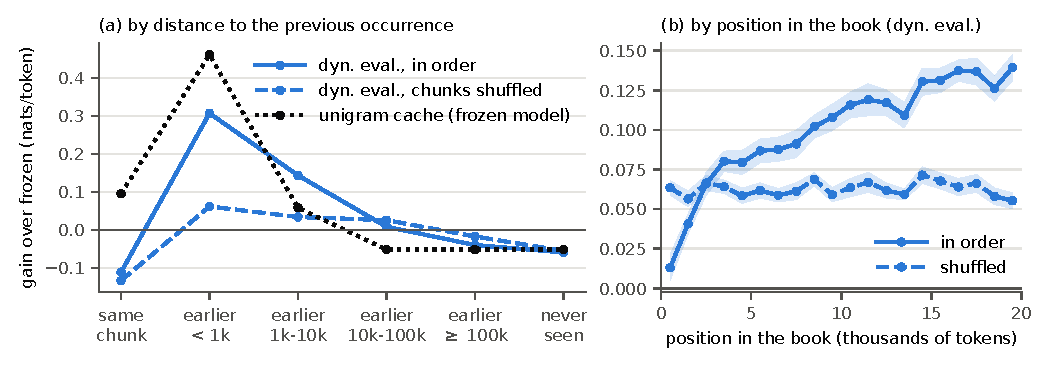
\includegraphics[width=0.97\textwidth]{distance_position.pdf}
\caption{Gain over frozen Pythia-14M with plain SGD (lr $10^{-4}$). (a) By distance to the token's previous occurrence, for dynamic evaluation in order and shuffled and for the unigram cache. (b) By position in the book, mean over the 24 books that follow a book switch, $\pm 1$ SE over books.}
\label{fig:distance}
\end{figure*}

The memory is tied mostly to the current book.
Splitting the earlier-chunk bins by whether the previous occurrence was in the same book, the locality gain between 1k and 10k tokens back is \localityTenKSamePM{} for same-book tokens and \localityTenKEarlierPM{} for earlier-book ones; between 10k and 100k, same-book tokens keep \localityHundredKSamePM{} and earlier-book tokens have none (\localityHundredKEarlierPM{}).
It is also more than a count cache.
A cache of recent token counts mixed into the frozen model ($p = 0.95\, p_\text{model} + 0.05\, p_\text{cache}$, counts halving every 1k tokens) is the better copier less than 1k tokens back (\gainUnigramOneKPM{} against \gainInOrderOneK{}), but from 1k tokens on dynamic evaluation gains more (\gainInOrderTenK{} against \gainUnigramTenKPM{} between 1k and 10k; paired difference \inOrderMinusUnigramTenKPM{}), and \inOrderMinusUnigramAllPM{} more overall.

\subsection{Locality as a variable}\label{sec:levels}

A cache should help more the longer the input stays on the same material.
The gain falls at every step of decreasing locality (Fig.~\ref{fig:levels}): \levelLongPM{} on the long books, \levelKOnePM{} with $K=1$, \levelKFivePM{} with $K=5$, \levelKTwentyFivePM{} with $K=25$ and \levelShuffledPM{} shuffled.
On the main set the paired drops are \dropKFivePM{} from $K=1$ to $K=5$, \dropKTwentyFivePM{} from $K=5$ to $K=25$ and \dropShuffledPM{} from $K=25$ to shuffled, so interleaving only 5 books removes most of the in-order advantage.
The long stream covers mostly different text, so the step from it to $K=1$ is not paired.

\begin{figure}[t]
\centering
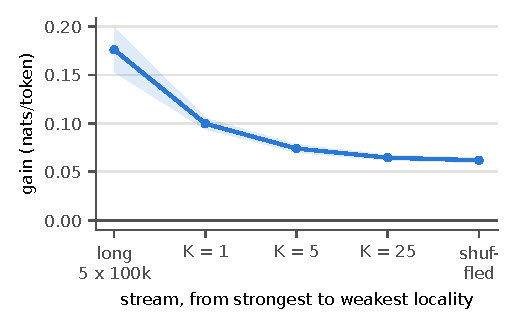
\includegraphics[width=\columnwidth]{locality_levels.pdf}
\caption{Gain over frozen Pythia-14M (plain SGD, all parameters, lr $10^{-4}$, $\pm 1$ SE over books) on streams of decreasing locality: 5 long books of 100k tokens, then the main set with books in order ($K=1$), 5 or 25 books interleaved, and shuffled.}
\label{fig:levels}
\end{figure}

\subsection{Where the memory lives}\label{sec:where}

If the memory sits in particular weights, updating only those should keep it.
We update one part of Pythia-14M at a time, each at its own learning rate (Table~\ref{tab:subsets}).
Freezing the output embedding costs little (\minusFullNoOutputAllPM{} overall against all parameters).
The output embedding alone is a short-range cache: \gainOutputOneKPM{} less than 1k tokens back but \gainOutputTenKSamePM{} between 1k and 10k (same book), and the largest loss on never-seen tokens (\gainOutputNeverPM{}).
Attention alone keeps less of the long-range gain (\gainAttentionTenKSamePM{} between 1k and 10k, same book).
Updating only the MLPs (lr $3\times10^{-4}$) gains more than updating all parameters: \gainMlpOneKPM{} against \gainInOrderOneK{} less than 1k tokens back (paired difference \minusFullMlpOneKPM{}) and \gainMlpAllPM{} against \gainInOrderAll{} overall.
One layer's MLP alone keeps between \layerShareOneKMin{} and \layerShareOneKMax{} of the full learner's gain less than 1k tokens back; the strongest is layer \layerBest{} and the last layer is the weakest (Fig.~\ref{fig:layers}).

The MLP-only learner owes its larger gain to a stronger cache, not to better general adaptation: its locality gain is \mvfMlpLocOneKPM{} against \mvfFullLocOneKPM{} less than 1k tokens back (paired \mvfDiffLocOneKPM{}), while shuffled it gains slightly less overall (\mvfDiffShuffledAllPM{}).
It also forgets more WikiText (\mvfMlpWikiPM{} against \mvfFullWikiPM{}, paired \mvfDiffWikiPM{}), at a lower exchange rate (\mvfMlpExchange{} against \mvfFullExchange{}).
All parameters at its rate, $3\times10^{-4}$, are already worse on val-pick (\valPickAllHigh{} against \valPickAll{}); with plain SGD at 14M attention takes \shareAttnFourteen{} of the squared update norm, which may limit the step the full learner can use.

\begin{table}[t]
\caption{Gain over frozen Pythia-14M when only some parameters are updated with plain SGD, in reading order ($K=1$), each subset at its own val-pick learning rate ($\pm$ SE over books). Columns are distance bins; ``same book'': the previous occurrence is in the same book.}
\label{tab:subsets}
\centering\footnotesize\setlength{\tabcolsep}{3pt}
\resizebox{\columnwidth}{!}{% Rows 1-5 of tables/layers.tex (copy of ../paper/tables/layers.tex) without the parameter-count column.
\begin{tabular}{lrrrrr}
\toprule
updated & lr & all & $<$ 1k & \begin{tabular}[b]{@{}r@{}}1k-10k,\\same book\end{tabular} & \begin{tabular}[b]{@{}r@{}}never\\seen\end{tabular} \\
\midrule
all parameters & $10^{-4}$ & $+0.100_{\pm .006}$ & $+0.307_{\pm .011}$ & $+0.154_{\pm .008}$ & $-0.059_{\pm .013}$ \\
output emb.\ only & $3\!\times\!10^{-3}$ & $+0.072_{\pm .005}$ & $+0.252_{\pm .017}$ & $+0.072_{\pm .006}$ & $-0.143_{\pm .012}$ \\
all but output emb. & $10^{-4}$ & $+0.094_{\pm .005}$ & $+0.294_{\pm .011}$ & $+0.151_{\pm .009}$ & $-0.058_{\pm .013}$ \\
MLPs only & $3\!\times\!10^{-4}$ & $+0.107_{\pm .007}$ & $+0.415_{\pm .016}$ & $+0.175_{\pm .011}$ & $-0.077_{\pm .014}$ \\
attention only & $3\!\times\!10^{-4}$ & $+0.066_{\pm .005}$ & $+0.259_{\pm .011}$ & $+0.110_{\pm .009}$ & $-0.074_{\pm .014}$ \\
\bottomrule
\end{tabular}}
\end{table}

\begin{figure}[t]
\centering
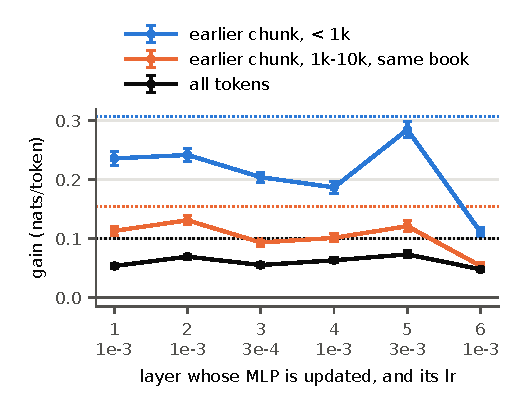
\includegraphics[width=\columnwidth]{layers.pdf}
\caption{Gain over frozen Pythia-14M with plain SGD when only one layer's MLP is updated, each at its own learning rate (below the layer number), $\pm 1$ SE over books. Dotted lines: all parameters at lr $10^{-4}$.}
\label{fig:layers}
\end{figure}

\subsection{Eviction}\label{sec:eviction}

If dynamic evaluation acts as a cache, reading other text should push a book out of memory (Fig.~\ref{fig:eviction}).
With plain SGD on all parameters at lr $10^{-4}$, the memory of A is \memoryZeroPM{} right after A1.
It halves after about \evictHalfLife{} tokens of other books and then declines slowly: \memoryTenKPM{} after 10k tokens, \memoryHundredKPM{} after 100k and \memoryThreeHundredKPM{} after 300k.
The snapshots never gain on the control book (\gainCZeroPM{} right after A1, between \gainCMin{} and \gainCMax{} later), so the decline is the loss of A rather than general adaptation catching up.
The memory is mostly about tokens that occurred in A1: rare tokens of A2 whose id occurs in A1 carry \memoryRareInPM{} after A1, other rare tokens \memoryRareNotInPM{}; the former halve after about \evictHalfLifeRare{} tokens.
A power law in $I$ fits better than an exponential with a floor ($\chi^2$ \fitChiPower{} against \fitChiExp{}, 4 degrees of freedom each), although the 7 points share the same 20 books.

\begin{figure*}[t]
\centering
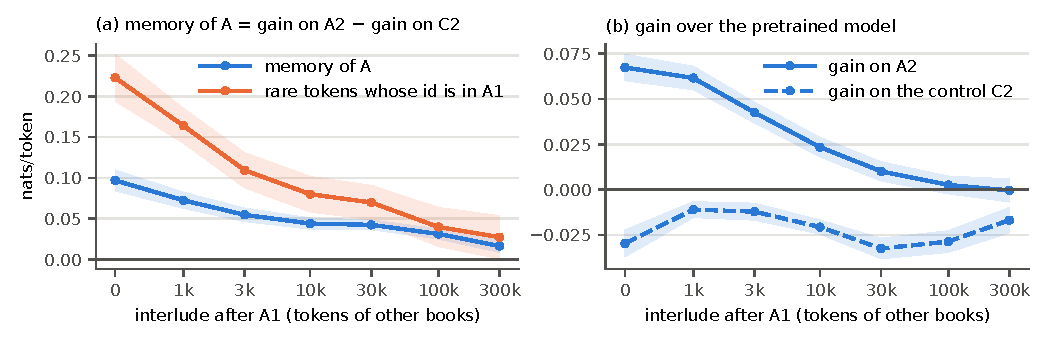
\includegraphics[width=0.97\textwidth]{eviction.pdf}
\caption{Eviction probed with frozen snapshots (Pythia-14M, plain SGD, all parameters, lr $10^{-4}$; mean of 20 books, bands $\pm 1$ SE over books), against the number of tokens of other books read after A1. (a) Memory of A (gain on A2 $-$ gain on the never-read control C2, same snapshot), and the same for rare tokens whose id occurs in A1. (b) Gain over the pretrained model on A2 and on C2.}
\label{fig:eviction}
\end{figure*}

\subsection{Collateral forgetting}\label{sec:forgetting}

A cache should leave the rest of memory intact.
We score frozen snapshots on text the learner never reads (Table~\ref{tab:forgetting}).
Reading the main set in order, Pythia-14M (plain SGD, lr $10^{-4}$) forgets \forgetWikiKOnePM{} nats/token on WikiText (pretrained loss \frozenWiki{}), about \wikiOverGainKOne{} times its gain on the stream (exchange rate \exchangeKOne{}), but loses nothing on the held-out PG-19 books (\forgetBooksKOnePM{}).
The shuffled learner forgets less on WikiText (\forgetWikiShuffledPM{}) and improves on the unseen books (\forgetBooksShuffledPM{}): the part of the gain that survives shuffling is adaptation to PG-19 text, and it carries over.
Reading in order forgets more than shuffled on both sets (\shMinusKOneWikiPM{} on WikiText, \shMinusKOneBooksPM{} on the books), at about the same exchange rate (\exchangeKOne{} and \exchangeShuffled{}).
Over the very long stream (800k tokens), forgetting on WikiText averages \veryLongWikiBookOne{} over the snapshots in the first book and \veryLongWikiBookTwo{}, \veryLongWikiBookThree{} and \veryLongWikiBookFour{} in the next three: it levels off after the first book, while the held-out books lose a little (\forgetBooksVeryLongPM{}).

\begin{table}[t]
\caption{Collateral forgetting of held-out text by Pythia-14M with plain SGD on all parameters (lr $10^{-4}$): snapshot loss $-$ pretrained loss, mean over the snapshots in the second half of the stream, $\pm$ SE over the WikiText chunks or the 6 held-out books; positive means knowledge lost. Stream gain: over the frozen loss on the stream, $\pm$ SE over books. Exchange rate = stream gain / forgetting on WikiText. Very long: 4 books of 200k tokens. $\dagger$: under 2 SE.}
\label{tab:forgetting}
\centering\footnotesize\setlength{\tabcolsep}{3pt}
% tables/forgetting.tex (copy of ../paper/tables/forgetting.tex) with shorter headers for one column.
\begin{tabular}{lrrrr}
\toprule
stream & \begin{tabular}[b]{@{}r@{}}stream\\gain\end{tabular} & \begin{tabular}[b]{@{}r@{}}forgetting,\\WikiText\end{tabular} & \begin{tabular}[b]{@{}r@{}}forgetting,\\held-out books\end{tabular} & \begin{tabular}[b]{@{}r@{}}exch.\\rate\end{tabular} \\
\midrule
$K=1$ & $+0.100_{\pm .006}$ & $+0.196_{\pm .006}$ & $-0.006_{\pm .010}^{\dagger}$ & 0.51 \\
shuffled & $+0.062_{\pm .003}$ & $+0.112_{\pm .004}$ & $-0.045_{\pm .008}$ & 0.55 \\
very long & $+0.170_{\pm .011}$ & $+0.268_{\pm .008}$ & $+0.052_{\pm .013}$ & 0.63 \\
\bottomrule
\end{tabular}
\end{table}

\subsection{Update rules, model size and a trade-off}\label{sec:rules}

We compare three update rules at three sizes, each at its own learning rate (Table~\ref{tab:rules}).
Over the first 40 chunks, plain SGD moves the MLP weights by \relMlpFourteen{} of their norm per step at 14M and \relMlpSeventy{} at 70M, about \mlpStepRatio{} times less, and at 70M attention takes \shareAttnSeventy{} of the squared update norm.
With plain SGD, Pythia-70M has almost no locality gain (\rLocOneKSgdSeventyPM{} less than 1k tokens back).
Normalized SGD more than doubles 70M's gain (paired difference \nsgdMinusSgdGainSeventyPM{}) and gives it some locality gain (\rLocOneKNsgdSeventyPM{}), far less than at 14M and 31M (\rLocOneKNsgdFourteenPM{} and \rLocOneKNsgdThirtyOnePM{}), which are the largest of any rule.
Adam has no cache at any size (locality gain less than 1k tokens back \rLocOneKAdamFourteenPM{}, \rLocOneKAdamThirtyOnePM{} and \rLocOneKAdamSeventyPM{}).
From 14M to 31M, plain SGD's locality gain does not change beyond noise (\locDiffThirtyOneFourteenOneKPM{} less than 1k tokens back), and the smaller model does not pay more general knowledge per nat of gain.

\begin{table*}[t]
\caption{Three update rules at three sizes, all parameters, each at its val-pick learning rate: gain with $K=1$ over each model's frozen loss and locality gain (in order $-$ shuffled, paired), $\pm$ SE over books; collateral forgetting on WikiText ($K=1$, second half of the stream, $\pm$ SE over chunks); exchange rate (stream gain / collateral forgetting on WikiText) in order and shuffled. $\dagger$: under 2 SE.}
\label{tab:rules}
\centering\footnotesize\setlength{\tabcolsep}{4pt}
\begin{tabular}{llrrrrrrr}
\toprule
size & rule & lr & gain, $K=1$ & loc. gain, $<$ 1k & loc. gain, all & \begin{tabular}[b]{@{}r@{}}collateral forgetting,\\WikiText\end{tabular} & exch. rate, $K=1$ & shuffled \\
\midrule
14M & plain SGD & $10^{-4}$ & $+0.100_{\pm .006}$ & $+0.245_{\pm .009}$ & $+0.038_{\pm .004}$ & $+0.196_{\pm .006}$ & 0.51 & 0.55 \\
 & Adam & $3\!\times\!10^{-6}$ & $+0.086_{\pm .005}$ & $-0.052_{\pm .009}$ & $-0.004_{\pm .004}^{\dagger}$ & $+0.141_{\pm .005}$ & 0.61 & 0.91 \\
 & normalized SGD & $10^{-4}$ & $+0.113_{\pm .008}$ & $+0.372_{\pm .011}$ & $+0.056_{\pm .006}$ & $+0.316_{\pm .008}$ & 0.36 & 0.29 \\
31M & plain SGD & $3\!\times\!10^{-4}$ & $+0.085_{\pm .005}$ & $+0.262_{\pm .010}$ & $+0.040_{\pm .004}$ & $+0.228_{\pm .005}$ & 0.37 & 0.31 \\
 & Adam & $3\!\times\!10^{-6}$ & $+0.070_{\pm .004}$ & $-0.070_{\pm .011}$ & $-0.007_{\pm .003}$ & $+0.137_{\pm .004}$ & 0.51 & 0.75 \\
 & normalized SGD & $10^{-4}$ & $+0.092_{\pm .007}$ & $+0.418_{\pm .013}$ & $+0.060_{\pm .005}$ & $+0.348_{\pm .006}$ & 0.26 & 0.13 \\
70M & plain SGD & $10^{-5}$ & $+0.025_{\pm .002}$ & $+0.016_{\pm .003}$ & $+0.004_{\pm .002}$ & $+0.010_{\pm .002}$ & 2.57 & 2.67 \\
 & Adam & $3\!\times\!10^{-7}$ & $+0.029_{\pm .002}$ & $-0.140_{\pm .010}$ & $-0.015_{\pm .002}$ & $+0.060_{\pm .003}$ & 0.47 & 0.68 \\
 & normalized SGD & $3\!\times\!10^{-6}$ & $+0.057_{\pm .004}$ & $+0.084_{\pm .006}$ & $+0.018_{\pm .003}$ & $+0.039_{\pm .002}$ & 1.48 & 1.52 \\
\bottomrule
\end{tabular}
\end{table*}

If the cache and general knowledge share the same weights, filling one should erode the other.
Placing every run with snapshots on these two axes (Fig.~\ref{fig:tradeoff}), the order within 14M is the same on both: Adam (\rLocOneKAdamFourteen{}, \rWikiAdamFourteen{}), plain SGD on all parameters (\rLocOneKSgdFourteen{}, \rWikiSgdFourteen{}), plain SGD on the MLPs only (\mvfMlpLocOneK{}, \mvfMlpWiki{}) and normalized SGD (\rLocOneKNsgdFourteen{}, \rWikiNsgdFourteen{}).
The same holds within 31M, and at 70M for plain and normalized SGD, but Adam at 70M forgets more than both (\rWikiAdamSeventyPM{}) with negative locality gain.
Across sizes the points do not lie on one curve: at 70M every rule forgets far less for a given locality gain.
With ten points, one seed and one model family, this is a consistent ordering within the settings we tried, not a law.

\begin{figure}[t]
\centering
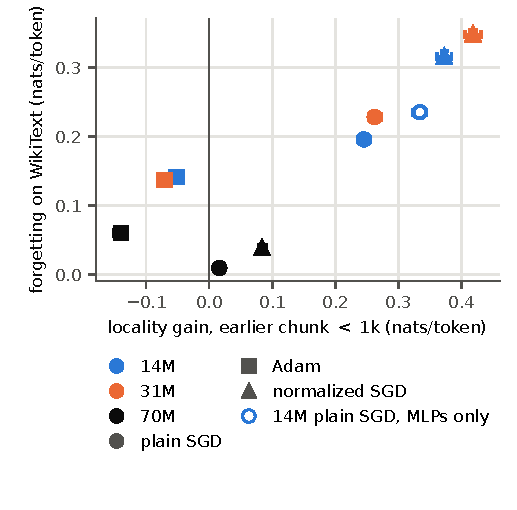
\includegraphics[width=\columnwidth]{tradeoff.pdf}
\caption{Locality gain less than 1k tokens back against collateral forgetting on WikiText ($K=1$, second half of the stream) for every run with snapshots: three update rules (marker) at three sizes (colour) on all parameters, and plain SGD on the MLPs only at 14M (open circle), each at its own learning rate. Bars: $\pm 1$ SE.}
\label{fig:tradeoff}
\end{figure}

\subsection{Long books and model size}\label{sec:long}

A cache is worth more the longer the material stays the same, and a small model might use it to approach a larger one (Table~\ref{tab:verylong}).
On the very long stream, Pythia-14M with plain SGD (lr $10^{-4}$) gains \vlGainOnlineFourteenPM{} over its frozen loss and closes \gapClosedFourteen{} of the gap to a frozen Pythia-31M.
The share grows from \gapFirstBin{} in the first 10k tokens of a book to \gapPeak{} between \gapPeakBin{} tokens, and is \gapLastBin{} in the last 10k; frozen 31M stays ahead overall (\vlFrozenThirtyOneAheadPM{}).
Pythia-31M with dynamic evaluation (lr $3\times10^{-4}$) gains about as much (\vlOnlineMinusFrozenThirtyOnePM{} over its frozen loss), stays ahead of 14M with dynamic evaluation, and does not reach a frozen Pythia-70M (\vlFrozenSeventyAheadPM{} behind).

\begin{table}[t]
\caption{Four PG-19 books of 200k tokens, read book after book: loss, gain over frozen Pythia-14M ($\pm$ SE over 4 books, paired) and share of the gap between frozen 14M and frozen 31M closed. Dynamic evaluation: plain SGD on all parameters.}
\label{tab:verylong}
\centering\footnotesize\setlength{\tabcolsep}{3pt}
\resizebox{\columnwidth}{!}{\begin{tabular}{lrrr}
\toprule
run & loss & gain over frozen 14M & share of 14M-31M gap \\
\midrule
frozen 14M & 4.419 &  &  \\
14M dyn.\ eval., lr $10^{-4}$ & 4.249 & $+0.170_{\pm .011}$ & 49\% \\
frozen 31M & 4.069 & $+0.351_{\pm .010}$ & 100\% \\
31M dyn.\ eval., lr $3\!\times\!10^{-4}$ & 3.901 & $+0.518_{\pm .013}$ & 148\% \\
frozen 70M & 3.846 & $+0.573_{\pm .013}$ & 163\% \\
\bottomrule
\end{tabular}}
\end{table}

\section{Discussion and limitations}

Dynamic evaluation helps more when the input has locality: the gain from more than 1k tokens back mostly disappears when the chunks are shuffled, and the overall gain falls at every step from long books to shuffled chunks.
The memory it builds is evicted as a cache's would be, halving after a few thousand tokens of other books with a long tail.
Unlike a cache, however, filling it overwrites general knowledge outside the domain, about twice the gain on the stream, and within 14M and 31M every setting we tried moved cache and collateral forgetting together, so no knob tested here separates the two.
The effect is not larger in the smaller model, at least between 14M and 31M, and 70M has less cache, depending on the update rule and the step it allows.
Nor can a small model with dynamic evaluation replace a larger one at these sizes: on long books it is worth about half the step from 14M to 31M, but 31M gains as much from it.

Our experiments are deliberately small: a single seed of three sizes of one model family reading PG-19, with WikiText as the out-of-domain reference.
Whether the behaviour holds in larger models and on other inputs with locality, such as code bases and long conversations, remains to be tested, as does repeating the analysis across pretraining seeds.
Scoring each chunk without earlier context isolates the memory in the weights; a practical assessment needs baselines with the full context window and with matched compute.
Since the cache and general knowledge compete for the same weights, a separate fast part on top of a frozen or slowly learning model could hold the recent context, and ablating Adam's momentum and per-weight normalization could show which property of the update rule a cache in the weights depends on.

\section{Conclusion}

A standard transformer updated by plain gradient steps has a cache in its weights: its benefit depends on locality (only \shuffledShareOneK{} of the gain less than 1k tokens back survives shuffling), it is tied to the book being read, it sits mostly in the MLPs, and other text evicts it after about \evictHalfLife{} tokens.
It is not a clean cache: knowledge of the same domain is preserved, but filling the cache costs about \wikiOverGainKOne{} nats of WikiText loss per nat gained.
Even so, on long books a 14M-parameter model with dynamic evaluation closes \gapClosedFourteen{} of the gap to a frozen model about twice its size.
Separating eviction from collateral forgetting could strengthen the cache and move towards small models that perform on the context at hand like larger ones.

\section*{Acknowledgements}
This work has been financed by Project PID2024-160996OB-I00, under grant agreement MICIU/\allowbreak AEI/\allowbreak 10.13039/\allowbreak 501100011033 and FEDER, UE, and by Generalitat de Catalunya (AGAUR) under grant agreement 2021-SGR-00478.

\section*{Data availability}
The code, the experimental results and the scripts that generate the tables and figures are available at \url{https://github.com/rtous/goldfish}.

\section*{Declaration of competing interest}
The authors declare that they have no known competing financial interests or personal relationships that could have appeared to influence the work reported in this paper.

\section*{Declaration of generative AI and AI-assisted technologies in the manuscript preparation process}
During the preparation of this work the authors used Claude (Anthropic) to assist with editing the text and preparing the manuscript for submission. After using this tool, the authors reviewed and edited the content as needed and take full responsibility for the content of the published article.

\bibliographystyle{model2-names}
\bibliography{manuscript}

\end{document}
